%%%%%%%%%%%%%%%%%%%%%%%%%%%%%%%%%%%%%%%%%
% Beamer Presentation
% LaTeX Template
% Version 1.0 (10/11/12)
%
% This template has been downloaded from:
% http://www.LaTeXTemplates.com
%
% License:
% CC BY-NC-SA 3.0 (http://creativecommons.org/licenses/by-nc-sa/3.0/)
%
%%%%%%%%%%%%%%%%%%%%%%%%%%%%%%%%%%%%%%%%%

%----------------------------------------------------------------------------------------
%	PACKAGES AND THEMES
%----------------------------------------------------------------------------------------

\documentclass{beamer}

\setbeamertemplate{caption}{\insertcaption}

\mode<presentation> {

% The Beamer class comes with a number of default slide themes
% which change the colors and layouts of slides. Below this is a list
% of all the themes, uncomment each in turn to see what they look like.

% \usetheme{default}
%\usetheme{AnnArbor}
%\usetheme{Antibes}
%\usetheme{Bergen}
% \usetheme{Berkeley}
%\usetheme{Berlin}
%\usetheme{Boadilla}
%\usetheme{CambridgeUS}
%\usetheme{Copenhagen}
%\usetheme{Darmstadt}
%\usetheme{Dresden}
% \usetheme{Frankfurt}
%\usetheme{Goettingen}
%\usetheme{Hannover}
\usetheme{Ilmenau}
%\usetheme{JuanLesPins}
%\usetheme{Luebeck}
% \usetheme{Madrid}
%\usetheme{Malmoe}  
%\usetheme{Marburg}
%\usetheme{Montpellier}
% \usetheme{PaloAlto}
%\usetheme{Pittsburgh}
%\usetheme{Rochester}
%\usetheme{Singapore}
%\usetheme{Szeged}
% \usetheme{Warsaw}

% Add slide numbers
\addtobeamertemplate{navigation symbols}{}{%
    \usebeamerfont{footline}%
    \usebeamercolor[fg]{footline}%
    \hspace{1em}%
    \insertframenumber/\inserttotalframenumber
}

% As well as themes, the Beamer class has a number of color themes
% for any slide theme. Uncomment each of these in turn to see how it
% changes the colors of your current slide theme.

%\usecolortheme{albatross}
%\usecolortheme{beaver}
%\usecolortheme{beetle} % nice
%\usecolortheme{crane}
%\usecolortheme{dolphin}
%\usecolortheme{dove} % nice
%\usecolortheme{fly}
%\usecolortheme{lily}
% \usecolortheme{orchid}
% \usecolortheme{rose}
%\usecolortheme{seagull}
%\usecolortheme{seahorse}
%\usecolortheme{whale} % nice
%\usecolortheme{wolverine}

%\setbeamertemplate{footline} % To remove the footer line in all slides uncomment this line
%\setbeamertemplate{footline}[page number] % To replace the footer line in all slides with a simple slide count uncomment this line

%\setbeamertemplate{navigation symbols}{} % To remove the navigation symbols from the bottom of all slides uncomment this line
}

\usepackage{graphicx} % Allows including images
\graphicspath{ {../imgs/} }

\usepackage{svg}
\usepackage{booktabs} % Allows the use of \toprule, \midrule and \bottomrule in tables
\usepackage{natbib}
\usepackage{physics}
\usepackage{siunitx}

%----------------------------------------------------------------------------------------
%	TITLE PAGE
%----------------------------------------------------------------------------------------

\title[Goodwin-Keen Economics]{An Analytic and Numerical Study on the Goodwin and Goodwin-Keen Economics Models} % The short title appears at the bottom of every slide, the full title is only on the title page

\author[Mathlings]{Romi Lifshitz \inst{1} \and Arthur M\'endez-Rosales \inst{2} \and Sara Saad \inst{3} \\\and Grant Forsythe \inst{4} \and Gheeda Mourtada \inst{4} \and Jacob Keffer \inst{5} }
\institute[McMaster University]{\inst{1} Department of Arts and Science, McMaster University \and %
                      \inst{2} Department of Engineering Physics, McMaster University \and %
                      \inst{3} Department of Electrical and Computer Engineering, McMaster University \and %
                      \inst{4} Department of Mathematics and Statistics, McMaster University \and %
                      \inst{5} Department of Chemistry and Chemical Biology, McMaster University}
                      
% \author{John Smith} % Your name
% \institute[UCLA] % Your institution as it will appear on the bottom of every slide, may be shorthand to save space
% {
% University of California \\ % Your institution for the title page
% \medskip
% \textit{john@smith.com} % Your email address
% }
\date{\today} % Date, can be changed to a custom date
% \today

\begin{document}

\begin{frame}
\titlepage % Print the title page as the first slide
\end{frame}

\begin{frame}
\frametitle{Overview} % Table of contents slide, comment this block out to remove it
\tableofcontents % Throughout your presentation, if you choose to use \section{} and \subsection{} commands, these will automatically be printed on this slide as an overview of your presentation
\end{frame}

%----------------------------------------------------------------------------------------
%	PRESENTATION SLIDES
%----------------------------------------------------------------------------------------

%------------------------------------------------

%------------------------------------------------
% \subsection{Subsection Example} % A subsection can be created just before a set of slides with a common theme to further break down your presentation into chunks
% 



%------------------------------------------------
\section{Introduction}
%------------------------------------------------
\begin{frame}
\frametitle{Introduction}
\large
\begin{itemize}
    \setlength\itemsep{2em}
    \item Are economies primarily stable?
    \item An introduction to internal factors of the Goodwin and Goodwin-Keen models.
    \item How can these models be used?
\end{itemize}
\normalsize
\end{frame}
%------------------------------------------------
\begin{frame}
\frametitle{Purpose of Study}
\large
\begin{block}{~}
\textbf{Studying the long-term equilibrium impact that endogenous economic variables have on the simplified macro-economy, modeled by the Goodwin model as well as the extensions made by Keen.}
\end{block}
\normalsize
\end{frame}
%------------------------------------------------



%------------------------------------------------
\section{Methods}
%------------------------------------------------
\begin{frame}
\frametitle{Goodwin Model}
The Goodwin model \citep{p4} describes the evolution of the employment rate $\lambda$ and the wage share $\omega$ as
\begin{equation}
\begin{split}
    \dot{\lambda} &= \lambda \cdot \left( \frac{1-\omega}{\nu} - \alpha - \beta - \delta \right), \\
    \dot{\omega} &= \omega \cdot (\Phi(\lambda) - \alpha).
\end{split}
\end{equation}
The Phillips curve connects the employment rate to the wage share. It is defined as
\begin{equation} \label{eq:keenPhil}
    \Phi(\lambda) = \frac{\Phi_1}{(1-\lambda)^2}-\Phi_0.
\end{equation}
\end{frame}
%------------------------------------------------
\begin{frame}
\frametitle{Jacobian of the Goodwin Model}
The Jacobian matrix for the Goodwin system of equations is defined by
\begin{equation} \label{eq:goodwinJ}
\LARGE
\mathbf J =
\begin{bmatrix}
    \pdv{\lambda}\dot{\lambda} & \pdv{\omega}\dot{\lambda}\\[0.8em]
    \pdv{\lambda}\dot{\omega} &  \pdv{\omega}\dot{\omega}
\end{bmatrix}.
\end{equation}
\normalsize
\end{frame}
%------------------------------------------------
\begin{frame}
\frametitle{Model Parameters}
\vspace{-5mm}
\begin{table}
\caption{Table 1: Model Parameters \citep{p5}.}
\centering
\begin{tabular}{|c|c|}
\hline
\textbf{Parameter }     & \textbf{Value}         \\
\hline
$\alpha$                & $0.025$                       \\ [-0.3em]
$\beta$                 & $0.02$                        \\ [-0.3em]
$\delta$                & $0.01$                        \\ [-0.1em]\hline
~                       & ~                             \\ [-1em]
$\Phi_0$                & $\frac{0.04}{1-0.04^2}$       \\ [0.3em]
$\Phi_1$                & $\frac{0.04^3}{1-0.04^2}$     \\ [0.3em] \hline
$\kappa_0$              & $-0.0065$                     \\ [-0.2em]
$\kappa_1$              & $\mathrm e^{-5}$              \\ [-0.2em]
$\kappa_2$              & $20$                          \\ [-0.1em]\hline
$r$                     & $0.03$                        \\ [-0.3em]
$\nu$                   & $3$                           \\
\hline
\end{tabular}
\end{table}
\end{frame}

%------------------------------------------------
\begin{frame}
\frametitle{Methods Overview}
\begin{enumerate}
    \setlength\itemsep{2em}
    \item Generate symbolic model using SymPy Python Solver.
    \item Determine equilibrium points using symbolic equations.
    \item Calculate Jacobian and evaluate stability at equilibrium points.
    \item Validate equilibrium points by graphical and numerical means.
\end{enumerate}
\end{frame}

%------------------------------------------------
\begin{frame}
\frametitle{Goodwin-Keen Model}
The Goodwin-Keen model \citep{p8} describes the impact of three parameters on a simplified macro-economy as
\begin{equation}
\begin{split}
     \dot{\lambda} &= \lambda \cdot \left( \frac{\kappa(\pi)}{\nu} - \alpha - \beta - \delta \right),\\
    \dot{\omega} &= \omega \cdot (\Phi(\lambda) - \alpha),\\
    \dot{d} &= d\cdot\left(r-\frac{\kappa(\pi)}{\nu}+\delta\right)+\kappa(\pi)-(1-\omega), \\
    \pi &= 1-\omega-rd,
\end{split}
\end{equation}
where $\lambda$ is the employment rate, $\omega$ is wage share, and $d$ is private debt. $\kappa(\pi)$ now represents the non-linear rate of new investment, and $\pi$ represents the net profits share from capital investments.
\end{frame}
%------------------------------------------------
\begin{frame}
\frametitle{Jacobian of the Goodwin-Keen Model}
The Jacobian matrix for the system is now defined by 
\LARGE
\begin{equation} \label{eq:keenJ}
\mathbf J =
\begin{bmatrix}
    \pdv{\lambda}\dot{\lambda} & \pdv{\omega}\dot{\lambda} & \pdv{d}\dot{\lambda}\\[1em]
    \pdv{\lambda}\dot{\omega} & \pdv{\omega}\dot{\omega} & \pdv{d}\dot{\omega}\\[1em]
    \pdv{\lambda}\dot{d} & \pdv{\omega}\dot{d} & \pdv{d}\dot{d}
\end{bmatrix}.
\end{equation}
\normalsize
\end{frame}
%------------------------------------------------
\begin{frame}
\frametitle{Goodwin-Keen Model Sensitivity Analysis}
We ran 1000 simulations, across the following domains.
\begin{table}[]
\caption{Table 2: Sensitivity Simulation Domains.}
\centering
\begin{tabular}{|c|c|c|c|} \hline
  \textbf{Initial Condition} & \textbf{Lower Bound} & \textbf{Upper Bound} & \textbf{Step Size}  \\ \hline
$\lambda_0$ & $0.6$ & $1.0$ &  $0.044\overline 4$ \\ \hline
$\omega_0$ & $0.5$ & $1.0$ & $0.055\overline 5$  \\ \hline
$d_0$ & $0$ & $10$ & $1.11\overline 1$ \\
\hline
\end{tabular}
\end{table}
\end{frame}
%------------------------------------------------


\section{Analysis and Interpretation}
%------------------------------------------------
\begin{frame}
\frametitle{Goodwin Model Symbolic Solution}
The Jacobian of the Goodwin model is given by
\begin{equation} \label{eq:jac_good}
    \mathbf J = \begin{bmatrix}
        \frac{1-\omega}{\nu}-\alpha-\beta-\delta & -\frac{\lambda}{\nu}\\[1ex]
        \frac{2\Phi_1\omega}{(1-\lambda)^3} & \frac{\Phi_1}{(1-\lambda)^2}-\Phi_0-\alpha
\end{bmatrix}.
\end{equation}
Its long-term equilibria (disregarding the trivial solution) are given by
\begin{equation} \label{eq:goodwin_eqm}
\begin{split}
    (\lambda_\pm^\ast, \omega^\ast) &= \left(1\pm\sqrt{\frac{\Phi_1}{\alpha + \Phi_0}},\quad  1-\nu\cdot(\alpha + \beta + \delta)\right)
\end{split}.
\end{equation}
\end{frame}
%------------------------------------------------
\begin{frame}
\frametitle{Goodwin Model Symbolic Solution}
With the economically realistic equilibrium point
\begin{equation} \label{eq:goodwin_eqm_valid}
\begin{split}
    (\lambda^\ast, \omega^\ast) &= \left(1-\sqrt{\frac{\Phi_1}{\alpha + \Phi_0}},\quad  1-\nu\cdot(\alpha + \beta + \delta)\right)
\end{split},
\end{equation}
the system's Jacobian matrix yields the following eigenvalues
\begin{equation} \label{eq:goodwin_eig}
    \pm\sqrt 2\cdot\sqrt{\xi_1 - \xi_2},
\end{equation}
where
\footnotesize
\begin{equation}
\begin{split}
    \xi_1 &= \frac{\Phi_0 + \alpha}{\nu} + \frac{\sqrt{\Phi_1\cdot(\Phi_0 + \alpha)}(\Phi_0+\alpha)(\alpha+\beta+\delta)}{\Phi_1},\\
    \xi_2 &= \frac{\sqrt{\Phi_1\cdot(\Phi_0 + \alpha)}(\Phi_0 + \alpha)}{\Phi_1\nu} + (\Phi_0+\alpha)(\alpha+\beta+\delta).
\end{split}
\end{equation}
\normalsize
\end{frame}
%------------------------------------------------
\begin{frame}
\frametitle{Goodwin Model Symbolic Solution}
We can define two potential cases for these eigenvalues
\begin{equation*} \label{eq:goodwin_eig}
    \pm\sqrt 2\cdot\sqrt{\xi_1 - \xi_2},
\end{equation*}
\footnotesize
\begin{equation*}
\begin{split}
    \xi_1 &= \frac{\Phi_0 + \alpha}{\nu} + \frac{\sqrt{\Phi_1\cdot(\Phi_0 + \alpha)}(\Phi_0+\alpha)(\alpha+\beta+\delta)}{\Phi_1},\\
    \xi_2 &= \frac{\sqrt{\Phi_1\cdot(\Phi_0 + \alpha)}(\Phi_0 + \alpha)}{\Phi_1\nu} + (\Phi_0+\alpha)(\alpha+\beta+\delta).
    \end{split}
\end{equation*}
\normalsize
\begin{enumerate}
    \item $\xi_1 > \xi_2$ Eigenvalues are \emph{real} and the system is unstable.
    \item $\xi_1 < \xi_2$ Eigenvalues are purely \emph{imaginary}, \emph{real} parts are 0, and the system converges to a limit cycle.
\end{enumerate}
\end{frame}
%------------------------------------------------
\begin{frame}
\frametitle{Behaviour of the Goodwin Model}
\begin{center}
\label{frequencyGraph}
% 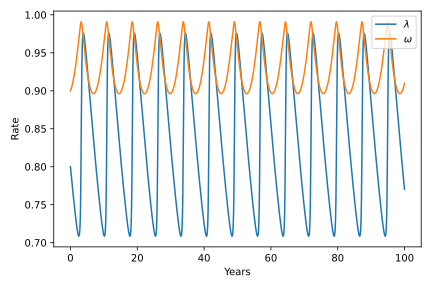
\includegraphics[scale=0.80]{goodwin.svg}
\includesvg[scale=0.6]{../imgs/goodwin_model.svg}
\end{center}
\end{frame}
%------------------------------------------------
\begin{frame}
\frametitle{Goodwin Equilibrium and Cyclical Behaviour}
\begin{center}
\label{frequencyGraph}
% 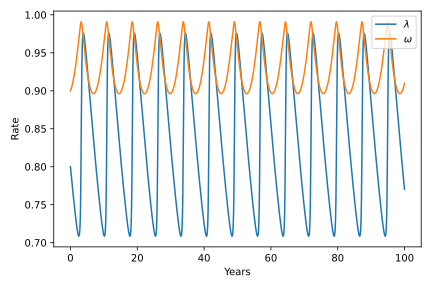
\includegraphics[scale=0.80]{goodwin.svg}
\includesvg[scale=0.45]{../imgs/goodwin_phase.svg}
\begin{equation*}
    (\lambda^\ast, \omega^\ast) = (0.968612, 0.835000).
\end{equation*}
\end{center}
\end{frame}
%------------------------------------------------
\begin{frame}
\frametitle{Goodwin-Keen Model Symbolic Solution}
The Jacobian matrix for the Goodwin-Keen model makes use of both \eqref{eq:keenPhil} and 
\begin{equation*} \label{eq:keenKappa}
    \kappa=\kappa(\pi) = \kappa_0 + \kappa_1\mathrm e^{\kappa_2\pi}.
\end{equation*}
Before we present the matrix, we note the use of the notational simplification
\begin{equation*}
    \kappa^\prime = -\pdv{\kappa}{\omega} = -\frac{1}{r}\pdv{\kappa}{d} = \kappa_1\kappa_2\mathrm e^{\kappa_2\pi}.
\end{equation*}
\end{frame}

%------------------------------------------------
\begin{frame}
\frametitle{Goodwin-Keen Model Symbolic Solution}
Thus, the Jacobian matrix for the Goodwin-Keen model is given by
\begin{equation} \label{eq:jac_keen}
    \mathbf J = %
    \begin{bmatrix}
        \frac{\kappa-\nu(\alpha+\beta+\delta)}{\nu} & -\frac{\lambda\kappa^\prime}{\nu} & -\frac{\lambda r\kappa^\prime}{\nu} \\[0.5em]
        \frac{2\Phi_1\omega}{(1-\lambda)^3} & \frac{\Phi_1}{(1-\lambda)^2}-\Phi_0-\alpha & 0\\[0.5em]
        0 & \frac{(d-\nu)\kappa^\prime+\nu}{\nu} & \frac{r\cdot(d-\nu)\kappa^\prime}{\nu}+ \delta + r
    \end{bmatrix}.
\end{equation}
\end{frame}
%------------------------------------------------
\begin{frame}
\frametitle{Goodwin-Keen Plot}
\begin{center}
\label{frequencyGraph}
% 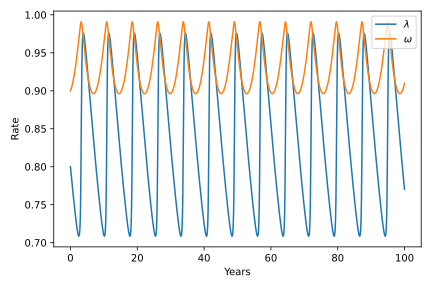
\includegraphics[scale=0.80]{goodwin.svg}
\includesvg[scale=0.6]{../imgs/keen_model.svg}
\end{center}
\end{frame}
%------------------------------------------------
\begin{frame}
\frametitle{Goodwin-Keen ``Good'' Equilibrium}
\begin{center}
\label{frequencyGraph}
% 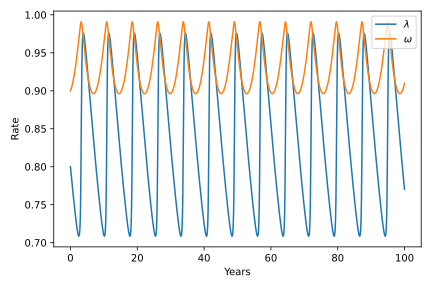
\includegraphics[scale=0.80]{goodwin.svg}
\includesvg[scale=0.6]{../imgs/keen_phase.svg}
\end{center}
\end{frame}
%------------------------------------------------
\begin{frame}
\frametitle{Goodwin-Keen Basin of Attraction}
\begin{center}
\label{frequencyGraph}
% 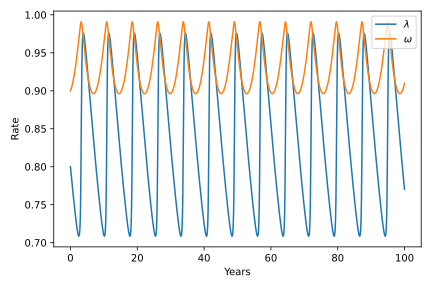
\includegraphics[scale=0.80]{goodwin.svg}
\includesvg[scale=0.6]{../imgs/keen_study.svg}
\end{center}
\end{frame}
%------------------------------------------------
\begin{frame}{Goodwin-Keen ``Good'' Equilibrium}
    \begin{figure}
        \includesvg[width=0.48\textwidth]{keen_model_conv.svg} % \hfill
        \includesvg[width=0.5\textwidth]{keen_phase_conv.svg}
    \end{figure}
    \begin{equation*}
        (\lambda^\ast, \omega^\ast, d^\ast) = (0.968612, 0.86053, 0.070191).
    \end{equation*}
\end{frame}
%------------------------------------------------
\begin{frame}{Goodwin-Keen ``Bad'' Equilibrium}
    \begin{figure}
        \includesvg[width=0.48\textwidth]{keen_model_div.svg} % \hfill
        \includesvg[width=0.5\textwidth]{keen_phase_div.svg}
    \end{figure}
    \begin{equation*}
        (\lambda^\times, \omega^\times, d^\times) = (0, 0, +\infty).
    \end{equation*}
\end{frame}
%------------------------------------------------
\begin{frame}{Model Comparison}
    \begin{minipage}[t]{0.5\linewidth}
    \textbf{The Goodwin Model}
    \begin{enumerate}
        \item Dynamically analogous to the prey-predator model.
        \item \emph{One} economically feasible equilibrium points.
        \item Has served as a stepping stone for more complete models \citep{p5, p9}.
    \end{enumerate}   
    \end{minipage}%
    \begin{minipage}[t]{0.5\linewidth}
    \textbf{The Goodwin-Keen Model}
    \setbeamertemplate{itemize items}{}
    \begin{enumerate}
        \item Capable of modeling a stable and unstable economy.
        \item \emph{Two} economically feasible equilibrium point.
        \item As an endogenous model, shows that economies can collapse solely due to internal factors \citep{p8}.
    \end{enumerate}
    \end{minipage}\par
\end{frame}




%------------------------------------------------
\section{Conclusion}

\begin{frame}{Conclusion}
    \begin{itemize}
        \setlength\itemsep{2em}
        \item Qualitative and mathematical presentation of Goodwin and Goodwin-Keen models.
        \begin{itemize}
            \item Employment and wage share.
            \item Employment, wage share, debt ratio, and net profits share.
        \end{itemize}
        \item Equilibrium found and behaviours plotted.
        \begin{itemize}
            \item Goodwin is too simplistic, but is foundational.
            \item Goodwin-Keen provides more realistic uses.
        \end{itemize}
    \end{itemize}
\end{frame}
\begin{frame}{Conclusion}
    \begin{itemize}
        \item Additional Works and Considerations
        \begin{itemize}
            \setlength\itemsep{2em}
            \item Full Keen model with all factors of \emph{Minsky Instability Hypothesis}
            \begin{itemize}
                \item \textit{Ponzi-esque} financing and regulatory effects.
            \end{itemize}
            \item Enviro-economical model constructed by \citet{p9}
            \begin{itemize}
                \item Connects the rising CO$_2$ levels to the Goodwin-Keen model, in hopes of an environmentally motivated economic model.
            \end{itemize}
            \item Real world impact of economic modelling, and its importance.
        \end{itemize}
    \end{itemize}
\end{frame}
%------------------------------------------------
\begin{frame}
\section{Acknowledgements}
\frametitle{Acknowledgements}
\large
\begin{block}{~}
\textbf{We would like to thank Nik Počuča (McMaster University) for encouraging us to think about and explore this problem. We would also like to thank Daniel Presta for useful discussions and invaluable feedback throughout the project.}
\end{block}
\normalsize
\end{frame}
%------------------------------------------------




\iffalse % START IGNORE CHUNK OF CODE
\section{Extra Slide Formats} % REMOVE THIS WHEN DONE!
\begin{frame}
% Equations will be in this format
\frametitle{Blocks of Highlighted Text}
\begin{block}{Block 1}
Lorem ipsum dolor sit amet, consectetur adipiscing elit. Integer lectus nisl, ultricies in feugiat rutrum, porttitor sit amet augue. Aliquam ut tortor mauris. Sed volutpat ante purus, quis accumsan dolor.
\end{block}

\begin{block}{Block 2}
Pellentesque sed tellus purus. Class aptent taciti sociosqu ad litora torquent per conubia nostra, per inceptos himenaeos. Vestibulum quis magna at risus dictum tempor eu vitae velit.
\end{block}

\begin{block}{Block 3}
Suspendisse tincidunt sagittis gravida. Curabitur condimentum, enim sed venenatis rutrum, ipsum neque consectetur orci, sed blandit justo nisi ac lacus.
\end{block}
\end{frame}

%------------------------------------------------
\begin{frame}
\frametitle{Multiple Columns}
\begin{columns}[c] % The "c" option specifies centered vertical alignment while the "t" option is used for top vertical alignment
\column{.45\textwidth} % Left column and width
\textbf{Heading}
\begin{enumerate}
\item Statement
\item Explanation
\item Example
\end{enumerate}

\column{.5\textwidth} % Right column and width
Lorem ipsum dolor sit amet, consectetur adipiscing elit. Integer lectus nisl, ultricies in feugiat rutrum, porttitor sit amet augue. Aliquam ut tortor mauris. Sed volutpat ante purus, quis accumsan dolor.
\end{columns}
\end{frame}

\begin{frame}
% Parameters will be in this format
\frametitle{Parameters}
\begin{table}
\begin{tabular}{l l l}
\toprule
\textbf{Treatments} & \textbf{Response 1} & \textbf{Response 2}\\
\midrule
Treatment 1 & 0.0003262 & 0.562 \\
Treatment 2 & 0.0015681 & 0.910 \\
Treatment 3 & 0.0009271 & 0.296 \\
\bottomrule
\end{tabular}
\caption{Table caption}
\end{table}
\end{frame}
%------------------------------------------------
\begin{frame}
\frametitle{Theorem}
\begin{theorem}[Mass--energy equivalence]
$E = mc^2$
\end{theorem}
\end{frame}
%------------------------------------------------
\begin{frame}[fragile] % Need to use the fragile option when verbatim is used in the slide
\frametitle{Verbatim}
\begin{example}[Theorem Slide Code]
\begin{verbatim}
\begin{frame}
\frametitle{Theorem}
\begin{theorem}[Mass--energy equivalence]
$E = mc^2$
\end{theorem}
\end{frame}\end{verbatim}
\end{example}
\end{frame}
%------------------------------------------------
\begin{frame}
\frametitle{Figure}
Uncomment the code on this slide to include your own image from the same directory as the template .TeX file.
%\begin{figure}
%\includegraphics[width=0.8\linewidth]{test}
%\end{figure}
\end{frame}
%------------------------------------------------
\begin{frame}[fragile] % Need to use the fragile option when verbatim is used in the slide
\frametitle{Citation}
An example of the \verb|\cite| command to cite within the presentation:\\~
This statement requires citation \cite{p1}.
\end{frame}
\fi % END IGNORE CHUNK OF CODE
%------------------------------------------------




%------------------------------------------------
\begin{frame}[allowframebreaks]{References}
\footnotesize{
\begin{thebibliography}{99} % Beamer does not support BibTeX so references must be inserted manually as below

\scriptsize
\bibitem[Boldrin, 1990]{p1} Boldrin, Woodford (1990)
\newblock Equilibrium Models Displaying Endogenous Fluctuations and Chaos:  a Survey
\newblock \emph{Journal of Monetary Economics} 25(2), 189–222.

\bibitem[Flashcel, 2016]{p2} Flaschel, Landesmann (2016)
\newblock Mathematical Economics and the Dynamics of Capitalism: Goodwin’s Legacy Continued
\newblock \emph{Routledge Frontiers of Political Economy}.

\bibitem[Ganti, 2019]{p3} Akhilesh Ganti (2019)
\newblock Exogenous Growth Definition
\newblock \emph{Investopedia}.

\bibitem[Goodwin, 1982]{p4} Richard Goodwin (1982)
\newblock A Growth Cycle
\newblock \emph{Essays in Economic Dynamics} 165-170.

\bibitem[Grasseli, 2012]{p5} Grasseli, Lima, et al. (2012)
\newblock An Analysis of the Keen Model for Credit Expansion, Asset Price Bubbles and Financial Fragility
\newblock \emph{Mathematics and Financial Economics} 6(3), 191–210.

\bibitem[Harvie, 2000]{p6} David Harvie (2000)
\newblock Testing Goodwin: Growth Cycles in Ten OECD Countries
\newblock \emph{Cambridge Journal of Economics} 24(3), 349–376.

\bibitem[Hunter, 2007]{p7} John Hunter (2007)
\newblock Matplotlib:  A 2d graphics environment
\newblock \emph{Computing in Science Engineering} 9(3), 90–95.

\bibitem[Keen, 1995]{p8} Steve Keen (1995)
\newblock Finance and Economic Breakdown:  Modeling Minsky’s ``Financial Instability Hypothesis''
\newblock \emph{Journal of Post Keynesian Economics} 7(4), 607–635.

\bibitem[{Giraud, et al.}, 2018]{p9} Geraud, et al. (2018)
    \newblock Coping with collapse: a stock-flow consistent monetary macrodynamics of global warming
    \newblock \emph{Ecological Economics}, 147, 383-398

% Sympy
\bibitem[Meurer, 2017]{p1} Meurer, et al. (2017)
\newblock Sympy:  Symbolic Computing in Python

\bibitem[Maheswari, 2015]{p1} Aditya Maheshwari (2015)
\newblock An Empirical Study of Goodwin Growth Models
\newblock \emph{PhD Thesis}

\bibitem[Minsky, 1992]{p1} Hyman Minsky (1992)
\newblock The Financial Instability Hypothesis
\newblock \emph{The Jerome Levy Economics Institue Working Paper} (74).

\bibitem[Moura Jr, 2013]{p1} Newton Moura Jr (2013)
\newblock Testing the Goodwin Growth-Cycle Macroeconomic Dynamics in Brazil
\newblock \emph{Physica A: Statistical Mechanics and its Applications} 392(9), 2088–2103.

\bibitem[Rossum, 1995]{p1} Guido Rossum (1995)
\newblock Python Reference Manual
\newblock \emph{CWI}

% Scipy
\bibitem[Virtanen, 2020]{p1} Pauli Virtanen, et al. (2020)
\newblock SciPy 1.0: Fundamental Algorithms for Scientific Computing in Python
\newblock \emph{Nature Methods} 17, 261-272.

% Numpy
\bibitem[Harris, 2020]{p1} Harris, et al. (2020)
\newblock Array Programming with NumPy
\newblock \emph{Nature} 6, 357-362.

% Pandas
\bibitem[McKinney, 2010]{p1} Wes McKinney (2010)
\newblock Data Structures for Statistical Computing in Python

\bibitem[Weitzman, 1983]{p1} Martin Weitzman (1983)
\newblock Some  Macroeconomic  Implications  of  Alternative  Compensation Systems
\newblock \emph{The Economic Journal } 93(372), 763–783.
\normalsize

\end{thebibliography}
}
\end{frame}

%------------------------------------------------

\begin{frame}
\Huge{\centerline{FIN}}
\end{frame}

%----------------------------------------------------------------------------------------

\end{document} 